\section{Results}




\subsection{Probability distribution}

The probability distribution of energy (\cref{fig:distribution}) shows that
at low temperature almost all of the states are in a low energy state.
As the temperature and the variance increases the distribution becomes more
spread out.

\begin{figure}[H]
  \centering
  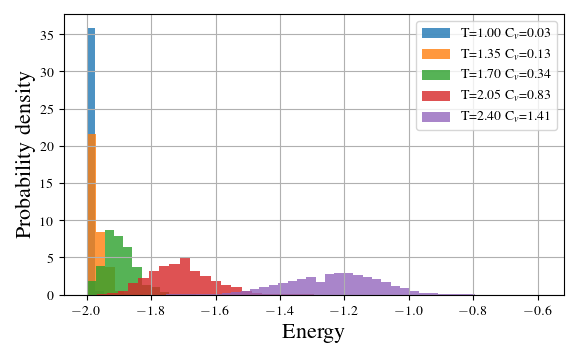
\includegraphics[width=\textwidth]{../figures/distribution.png}
  \caption{Probability distribution of energy, scaled with number of spins. L=20}
  \label{fig:distribution}
\end{figure}


\subsection{Phase transitions}

We did a production run to look for signs of phase transitions with T $\in
\brak{2.0,2.8}$, dT = \num{4e-3}, L $\in \brak{40,60,80,100}$, and \num{1e6} MC
cycles.
The results (\cref{fig:phase}) indicated a phase transition for T $\in
\brak{2.2,2.35}$. The simulations with higher grid size exhibits sharper
changes, meaning that they capture the phase transition better.


\begin{figure}[ht]
  \begin{subfigure}[t]{.5\textwidth} % top align
    \centering
    % include first image
    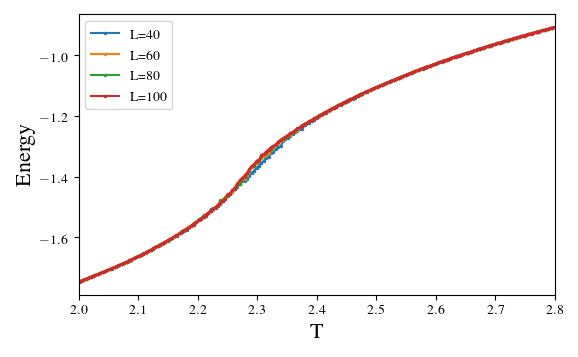
\includegraphics[width=\linewidth]{../figures/phase_E.png}
    \caption{Put your sub-caption here
    Put your sub-caption here
    Put your sub-caption here
    Put your sub-caption here}
    \label{fig:sub-first}
  \end{subfigure}
  \hfill
  \begin{subfigure}[t]{.5\textwidth}
    \centering
    % include second image
    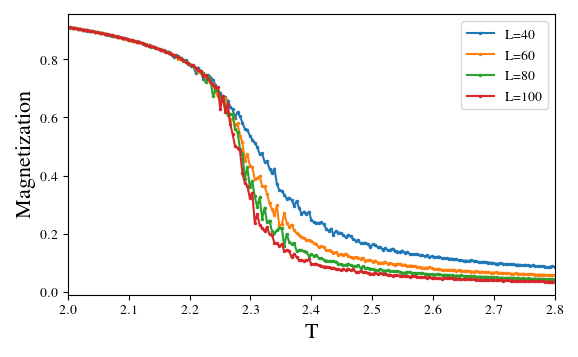
\includegraphics[width=\linewidth]{../figures/phase_Mabs.png}
    \caption{Put your sub-caption here}
    \label{fig:sub-second}
  \end{subfigure}
  \hfill
  \newline
  \begin{subfigure}[t]{.5\textwidth}
    \centering
    % include second image
    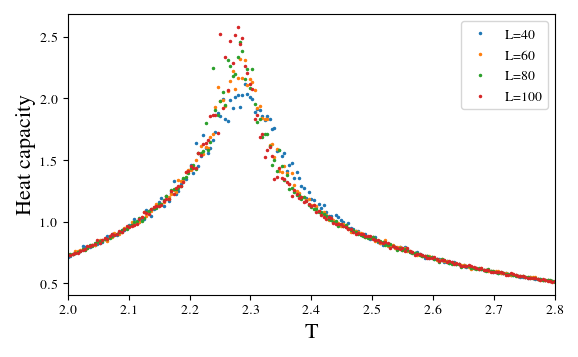
\includegraphics[width=\linewidth]{../figures/phase_cv.png}
    \caption{Put your sub-caption here}
    \label{fig:sub-second}
  \end{subfigure}
  \begin{subfigure}[t]{.5\textwidth}
    \centering
    % include second image
    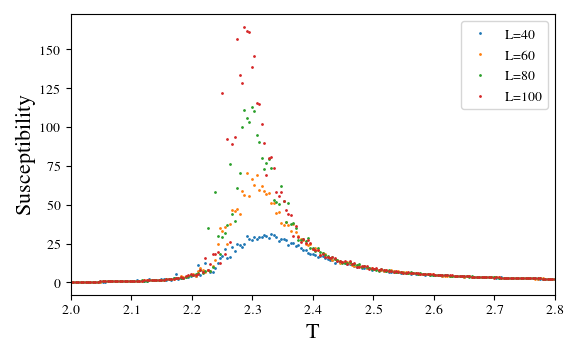
\includegraphics[width=\linewidth]{../figures/phase_suscept.png}
    \caption{Put your sub-caption here}
    \label{fig:sub-second}
  \end{subfigure}
\caption{Runs with T $\in \brak{2.0,2.8}$, dT = \num{4e-3} and
\num{1e6} MC cycles}
\label{fig:phase}
\end{figure}

To better capture the peaks of $C_v$ and $\chi$ we did another
run with dT = \num{5e-4} for T $\in \brak{2.2, 2.35}$.
 We fitted fourth order polynomials to $C_v$ and found
the critical temperature Tc$_{L}$ for each grid size.
Using the finite size scaling relation
\cref{eq:scaling} with $\nu$ = 1, we estimated $T_c(L=\infty)$
by doing a linear
regression with the four different T$_c$(L), using $1/L$ as the independent
variable, and extracting the intercept.
\footnote{Implemented in critical\_temperature.py}. The results are shown in
\cref{tab:results}.

 \begin{equation}
   \label{eq:scaling}
   T_C(L=\infty) = T_C(L) - aL^{-1/\nu}
 \end{equation}



 % This gave us the result of $Tc=2.26709 \pm 0.00237$.
 % Comparing with the analytical solution gave us the relative error
 % \cref{eq:analytical} $\epsilon_r = 0.00092$ with the 99\% confidence interval
 % $\brak{0.00012,0.00197}$.

 \begin{table}[htp]
 \centering
 \begin{tabular}{|l|l|l|ll}
 \cline{1-3}
                &        & 99\% confidence interval  &  &  \\ \cline{1-3}
 T$_c(L=\infty)$          & 2.26709   & {[}2.26472,2.26946{]}     &  &  \\ \cline{1-3}
 Relative error & 9.243e-04 & {[}1.210e-04,1.970e-03{]} &  &  \\ \cline{1-3}
 \end{tabular}
 \caption{Estimations of the critical temperature. Relative errors obtained by
 comparison with Lars Onsager's analytical solution \cref{eq:analytical}.}
 \label{tab:results}
 \end{table}


\begin{equation}
  \label{eq:analytical}
  T_C(L=\infty) = \frac{2}{\ln(1 + \sqrt2)} \approx 2.269
\end{equation}






% \begin{figure}[H]
%   \centering
%   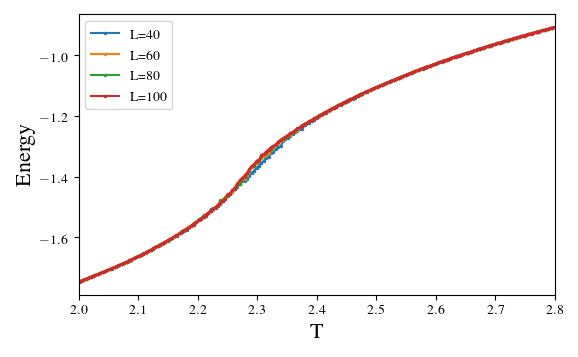
\includegraphics[width=\textwidth]{../figures/phase_E.png}
%   \caption{Mean energy. Some small differences between grid sizes. Run with T $\in \brak{2.0,2.8}$, dT = \num{4e-3} and
%   \num{1e6} MC cycles}
%   \label{fig:phase_E}
% \end{figure}
%
% \begin{figure}[H]
%   \centering
%   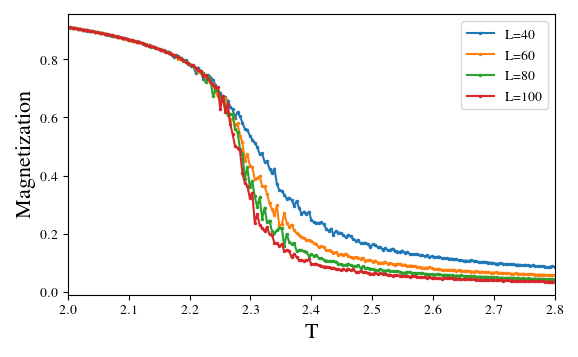
\includegraphics[width=\textwidth]{../figures/phase_Mabs.png}
%   \caption{Mean magnetisation.  Run with T $\in \brak{2.0,2.8}$, dT = \num{4e-3} and
%   \num{1e6} MC cycles}
%   \label{fig:phase_Mabs}
% \end{figure}
%
%
%
% \begin{figure}[H]
%   \centering
%   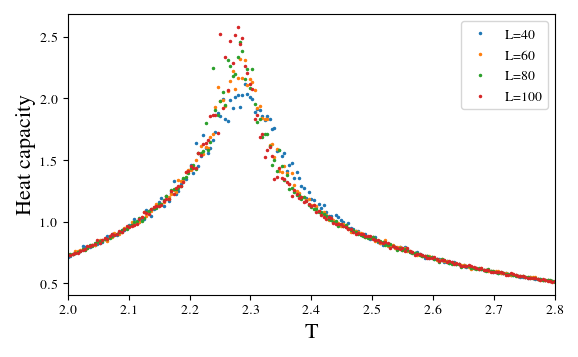
\includegraphics[width=\textwidth]{../figures/phase_cv.png}
%   \caption{Heat capacity. Run with T $\in \brak{2.0,2.8}$, dT = \num{4e-3} and
%   \num{1e6} MC cycles}
%   \label{fig:phase_cv}
% \end{figure}
%
%
% \begin{figure}[H]
%   \centering
%   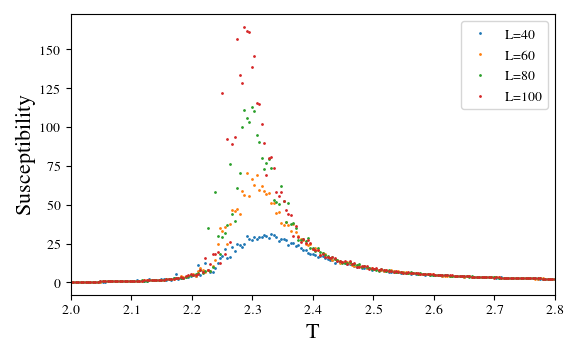
\includegraphics[width=\textwidth]{../figures/phase_suscept.png}
%   \caption{Susceptibility. Run with T $\in \brak{2.0,2.8}$, dT = \num{4e-3} and
%   \num{1e6} MC cycles}
%   \label{fig:phase_suscept}
% \end{figure}
